\subsection{Python语言简介}

\begin{frame}[standout] 第二节 \quad 操作系统和编程语言 \end{frame}

% 接下来,我们开始讲 第二节 操作系统和编程语言 的内容

\begin{frame}{Python语言的特点}
    \begin{figure}
        \centering
        
\includegraphics[width=8cm]{Images/Python.jpg}
    \end{figure}
    \small{
        \begin{itemize}
            \item Guido van Rossum在 1989 年创造了Python,在 1991 年将 Python 首次公开发行
            \item 跨平台、开源、解释型语言、高级语言
            \item 源代码可见
            \item 第三方包种类多, 可用底层语言(如C、Rust)重写关键代码
            \item 开发效率高,执行效率低
        \end{itemize}
    }
\end{frame}

% 在正式讲解操作系统之前, 我们先来简单了解一下 Python 的发展历史和特性
% 荷兰大叔 Guido van Rossum
% 在 1989 年创造了Python这门编程语言
% 并且在 1991 年将 Python 首次公开发行

% 经过了 30 年的发展,Python 已经成长为一个非常流行,跨平台,开源的编程语言
% Python 是一门解释型语言, 什么是解释型语言我们后面会讲
% 同时它是一门高级编程语言,拥有近似自然语言的表达能力

% Python 的源代码可见,不需要我们手动编译运行

% Python 也是一门胶水语言,能过融合其他高性能语言比如 C 的代码, 从而提高编写的程序性能,
% Python的开发效率很高, 由于表达能力强,内置工具包多等原因,
% 我们可以使用 Python快速搭建完成一个项目(大家注意看,他头发很多而且笑得很开心),

% 但是他的缺点也很明显,就是速度比较慢, 
% 而同样一个项目,使用如 C 语言去开发,可能开发时间就会很漫长,但是写出来的程序速度就会很快

\begin{frame}{Python语言的特点}
    \begin{itemize}
        \item Python 开发效率高,执行效率低 (科研,数据分析)
        \item C 开发效率低, 执行效率高 (高频量化交易)
        \begin{alertblock}{\small{执行效率对比}}
            \begin{itemize}
                \item  C \qquad \quad 10000行 \quad 0.01s
                \item  Java \quad \quad 1000行 \quad 0.05s
                \item  Python \quad 100行 \quad 0.1s
            \end{itemize}
        \end{alertblock}

    \end{itemize}
\end{frame}
% Python 的速度能有多慢呢, 我们列几个数字比较一下
% 当然不是严谨的,只是给大家一个概念
% C 或 Rust 等低级语言运行一万行代码,可能需要 0.01 秒
% -   提 JAVA 不提解释性语言
% 而 Java 运行 1000 行代码需要 0.05 秒 [注意,这里千万不要提 Java 的语言分类]
% 到了 Python 可能运行 100 行都需要 0.1 秒

% 但是不是说慢就一定不好啊,Python 100 行可以写出的程序,拿 C 来写可能就要写 1000 行
% 所以这是一个取舍,而对于生物信息学工作者来说,最重要的是能够快速实现想法,
% 等自己写的工具十分成熟和稳定了,才可能会考虑速度问题
\begin{frame}{Python擅长的领域}
    \begin{itemize}
        \item 爬虫
        \item Web后端开发
        \item 自动化运维、自动化测试
        \item 数据科学
        \item 机器学习
    \end{itemize}
\end{frame}

% 生物信息学是一个相对窄的领域, 那站在一个比较宏观的角度考虑, 
% Python 能做什么呢?
% 其实 Python 可以做的事情特别多
% 比如 Python 可以做爬虫, 网站后端开发,自动化运维和测试,数据科学和机器学习, 
% 那其实这里面的一些概念和方向大家可能不懂,或者不了解,
% 比如什么是爬虫什么是后端,什么是运维
% 其实, 在生物信息学上, Python 关于爬虫, 网页后端和其他方向都也有应用, 
% 我给大家举一些具体的例子感受一下

\begin{frame}{Python在生物信息学中的应用}
    \begin{columns}
        \column{0.4\textwidth}
        \begin{myoutline}[itemize]
            \1 数据获取(爬取UniProt)
                \2 \textcolor{lightgray}{爬虫}
            \1 \textcolor{lightgray}{Web前后端开发}
                \2 \textcolor{lightgray}{Django, Flask, 数据库\dots}
            \1 工作流程
                \2 Jupyterlab
                \2 \textcolor{lightgray}{Snakemake}
            \1 字符串处理
                \2 FASTA, FASTQ, BED-like, BAM/SAM
                \2 \underline{Biopython, Pysam}
            \1 数据分析机器学习
                \2 数据清洗, 数据分析, 可视化
                \2 \textcolor{lightgray}{特征工程, 机器学习}
        \end{myoutline}
        \column{0.6\textwidth}
        \begin{figure}
            \centering
            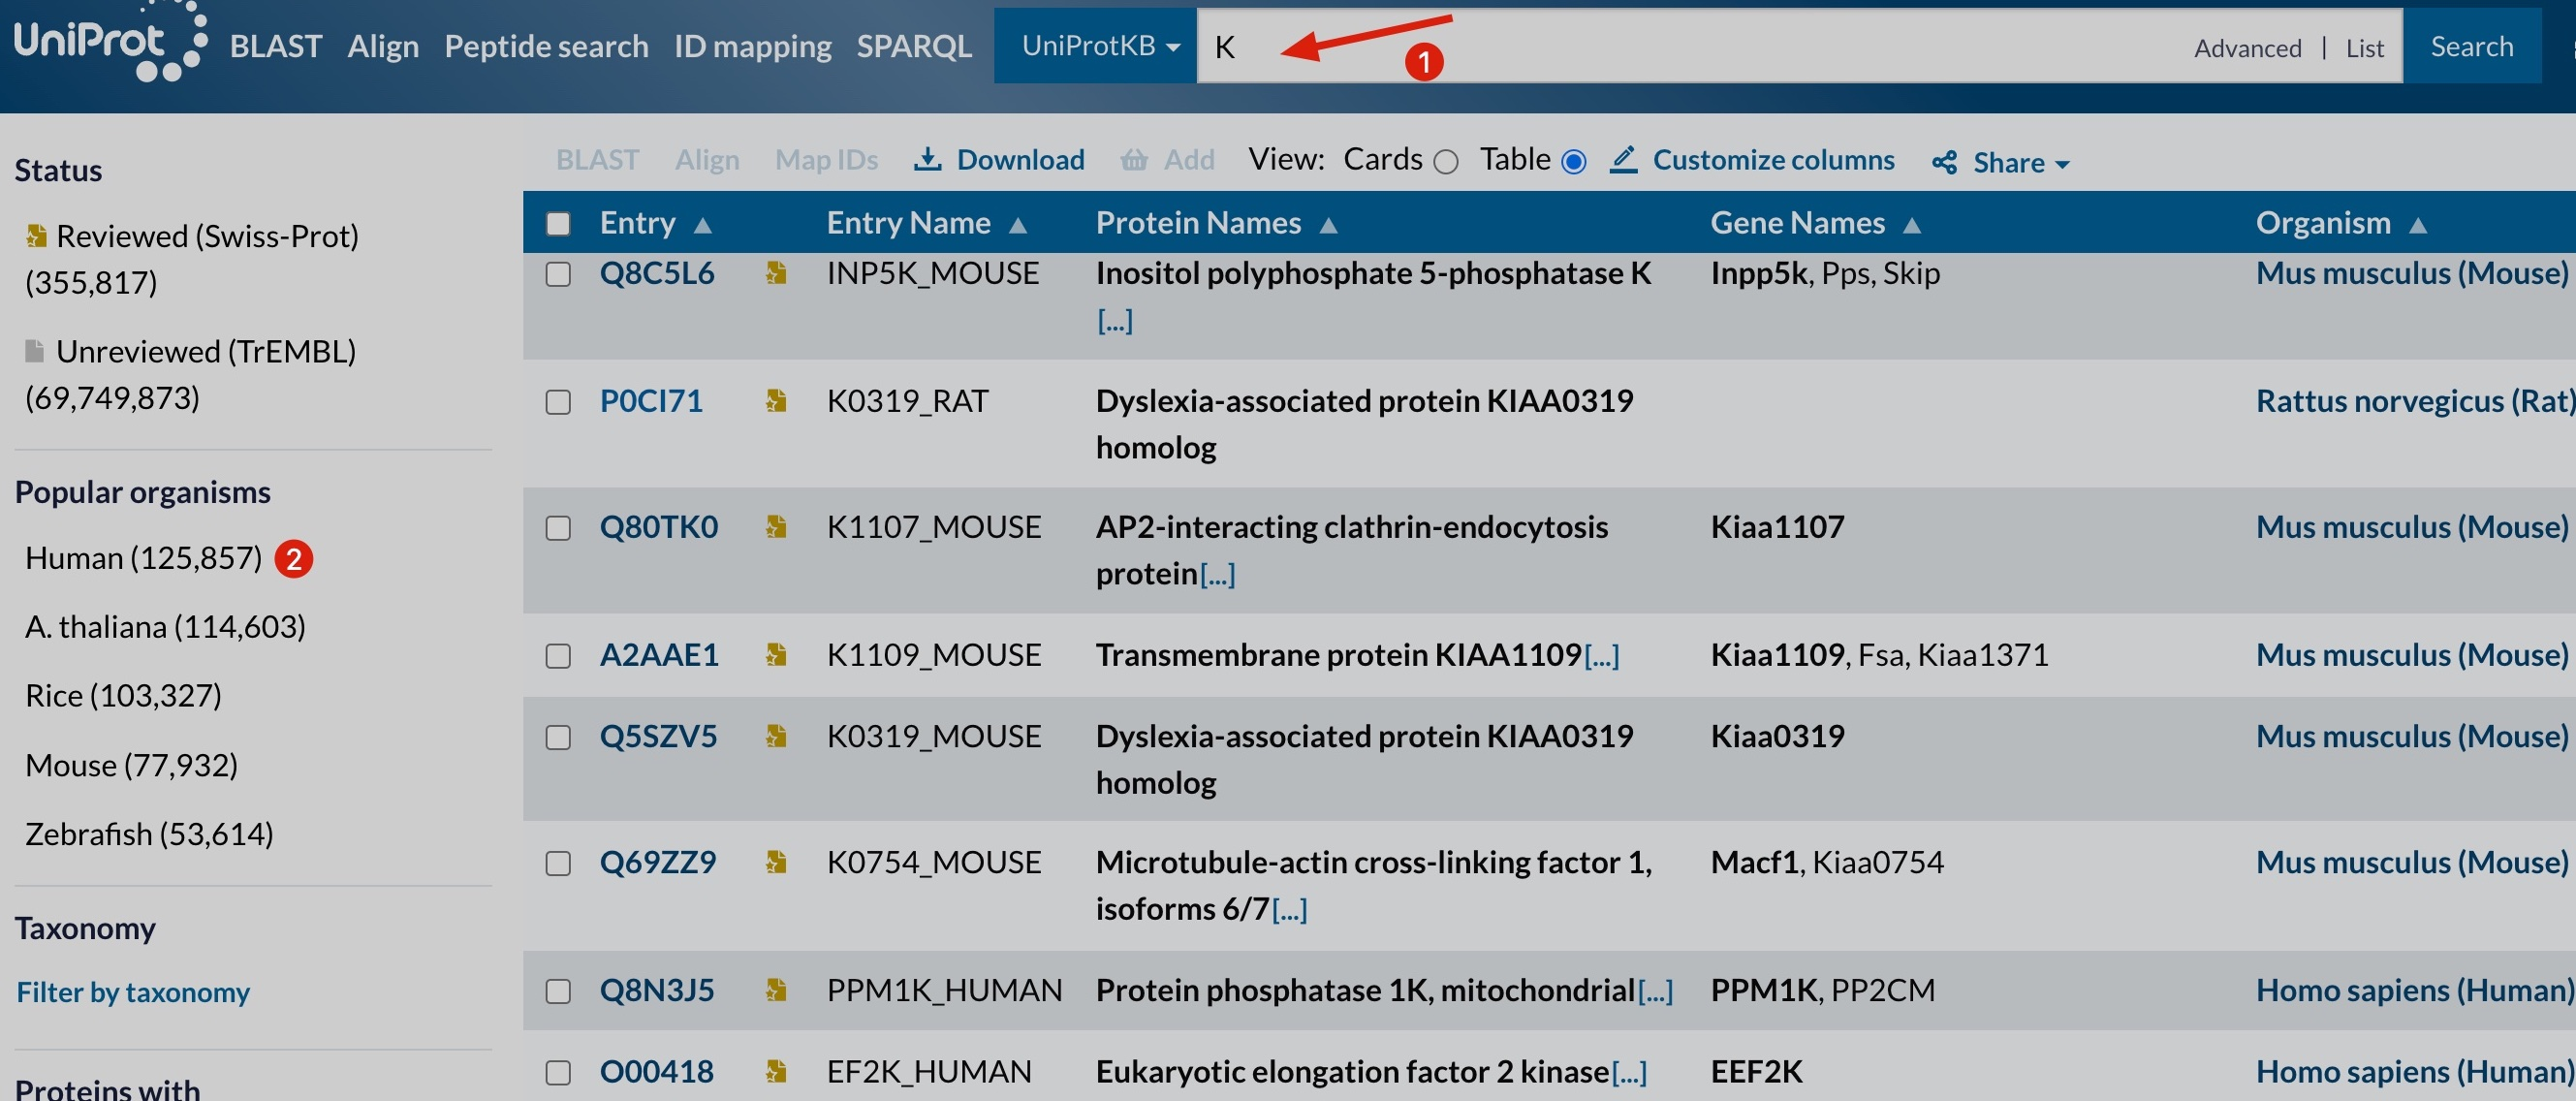
\includegraphics[width=8cm]{Images/uniprot.jpg}
            \caption{UniProt 蛋白数据库界面}
        \end{figure}
    \end{columns}

\end{frame}

% 比如,我们做数据分析,数据从哪里来,
% 假设要做一个蛋白结构预测的机器学习模型,那么我们需要大量的蛋白结构数据
% 一般我们获取一个蛋白结构可以去 UniProt 这个网页数据库中去检索然后使用鼠标操作下载
% 而如果我们需要几十万个蛋白,总不能一遍一遍点击,这样点到明年也下载不完
% 而爬虫就可以自动的帮我们打开浏览器操作网页,在很短的时间内访问并下载完这几十万个蛋白晶体结构
% 可以使用 Python开发爬虫来从公共网络中自动获取数据

\begin{frame}{Python在生物信息学中的应用}
    \begin{columns}
        \column{0.4\textwidth}
        \begin{myoutline}[itemize]
            \1 数据获取
                \2 \textcolor{lightgray}{爬虫}
            \1 \textcolor{lightgray}{Web前后端开发}
                \2 \textcolor{lightgray}{Django, Flask, 数据库\dots}
            \1 工作流程
                \2 Jupyterlab
                \2 \textcolor{lightgray}{Snakemake}
            \1 字符串处理
                \2 FASTA, FASTQ, BED-like, BAM/SAM
                \2 \underline{Biopython, Pysam}
            \1 数据分析机器学习 \\ (AlphaFold2$_{TensorFlow}$)
                \2 数据清洗, 数据分析, 可视化
                \2 \textcolor{lightgray}{特征工程, 机器学习}
        \end{myoutline}
        \column{0.6\textwidth}
        \begin{figure}
            \centering
            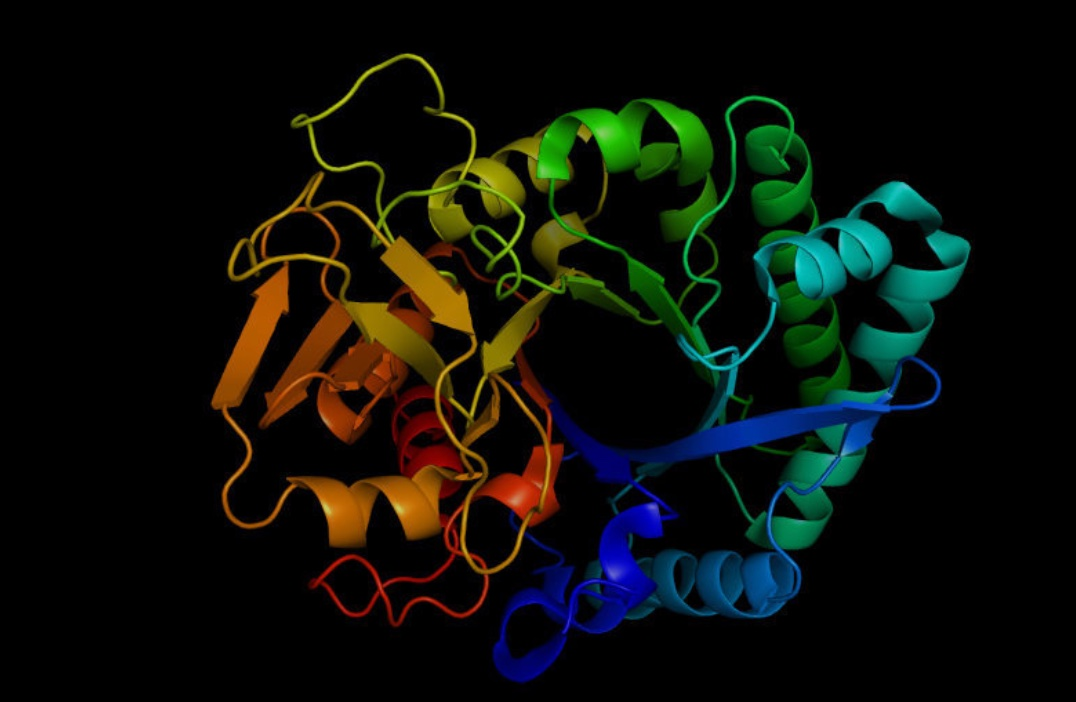
\includegraphics[width=8cm]{Images/alphafold.jpg}
            \caption{AlphaFold2 蛋白结构预测}
        \end{figure}
    \end{columns}
\end{frame}

% 那使用爬虫获取完这么多数据,就可以去使用机器学习模型进行结构预测,
% 现在大火的 AlphaFold2 就是一个预测蛋白结构的工具,
% 你可以把一个氨基酸序列输入给 AlphaFold2,经过计算它会告诉你这个氨基酸序列能折叠成什么样的三维结构,
% AlphaFold2 就是使用了大量晶体结构数据,
% 利用 Python 中很流行的一个机器学习框架,
% 叫 TensorFlow 的框架,经过大量数据的训练最终完成的机器学习模型

\begin{frame}{Python在生物信息学中的应用}
    \begin{columns}
        \column{0.4\textwidth}
        \begin{myoutline}[itemize]
            \1 数据获取
                \2 \textcolor{lightgray}{爬虫}
            \1 \textcolor{lightgray}{Web前后端开发} \\(AnnoLnc2)
                \2 \textcolor{lightgray}{Django, Flask, 数据库\dots}
            \1 工作流程
                \2 Jupyterlab
                \2 \textcolor{lightgray}{Snakemake}
            \1 字符串处理
                \2 FASTA, FASTQ, BED-like, BAM/SAM
                \2 \underline{Biopython, Pysam}
            \1 数据分析机器学习
                \2 数据清洗, 数据分析, 可视化
                \2 \textcolor{lightgray}{特征工程, 机器学习}
        \end{myoutline}
        \column{0.6\textwidth}
        \begin{figure}
            \centering
            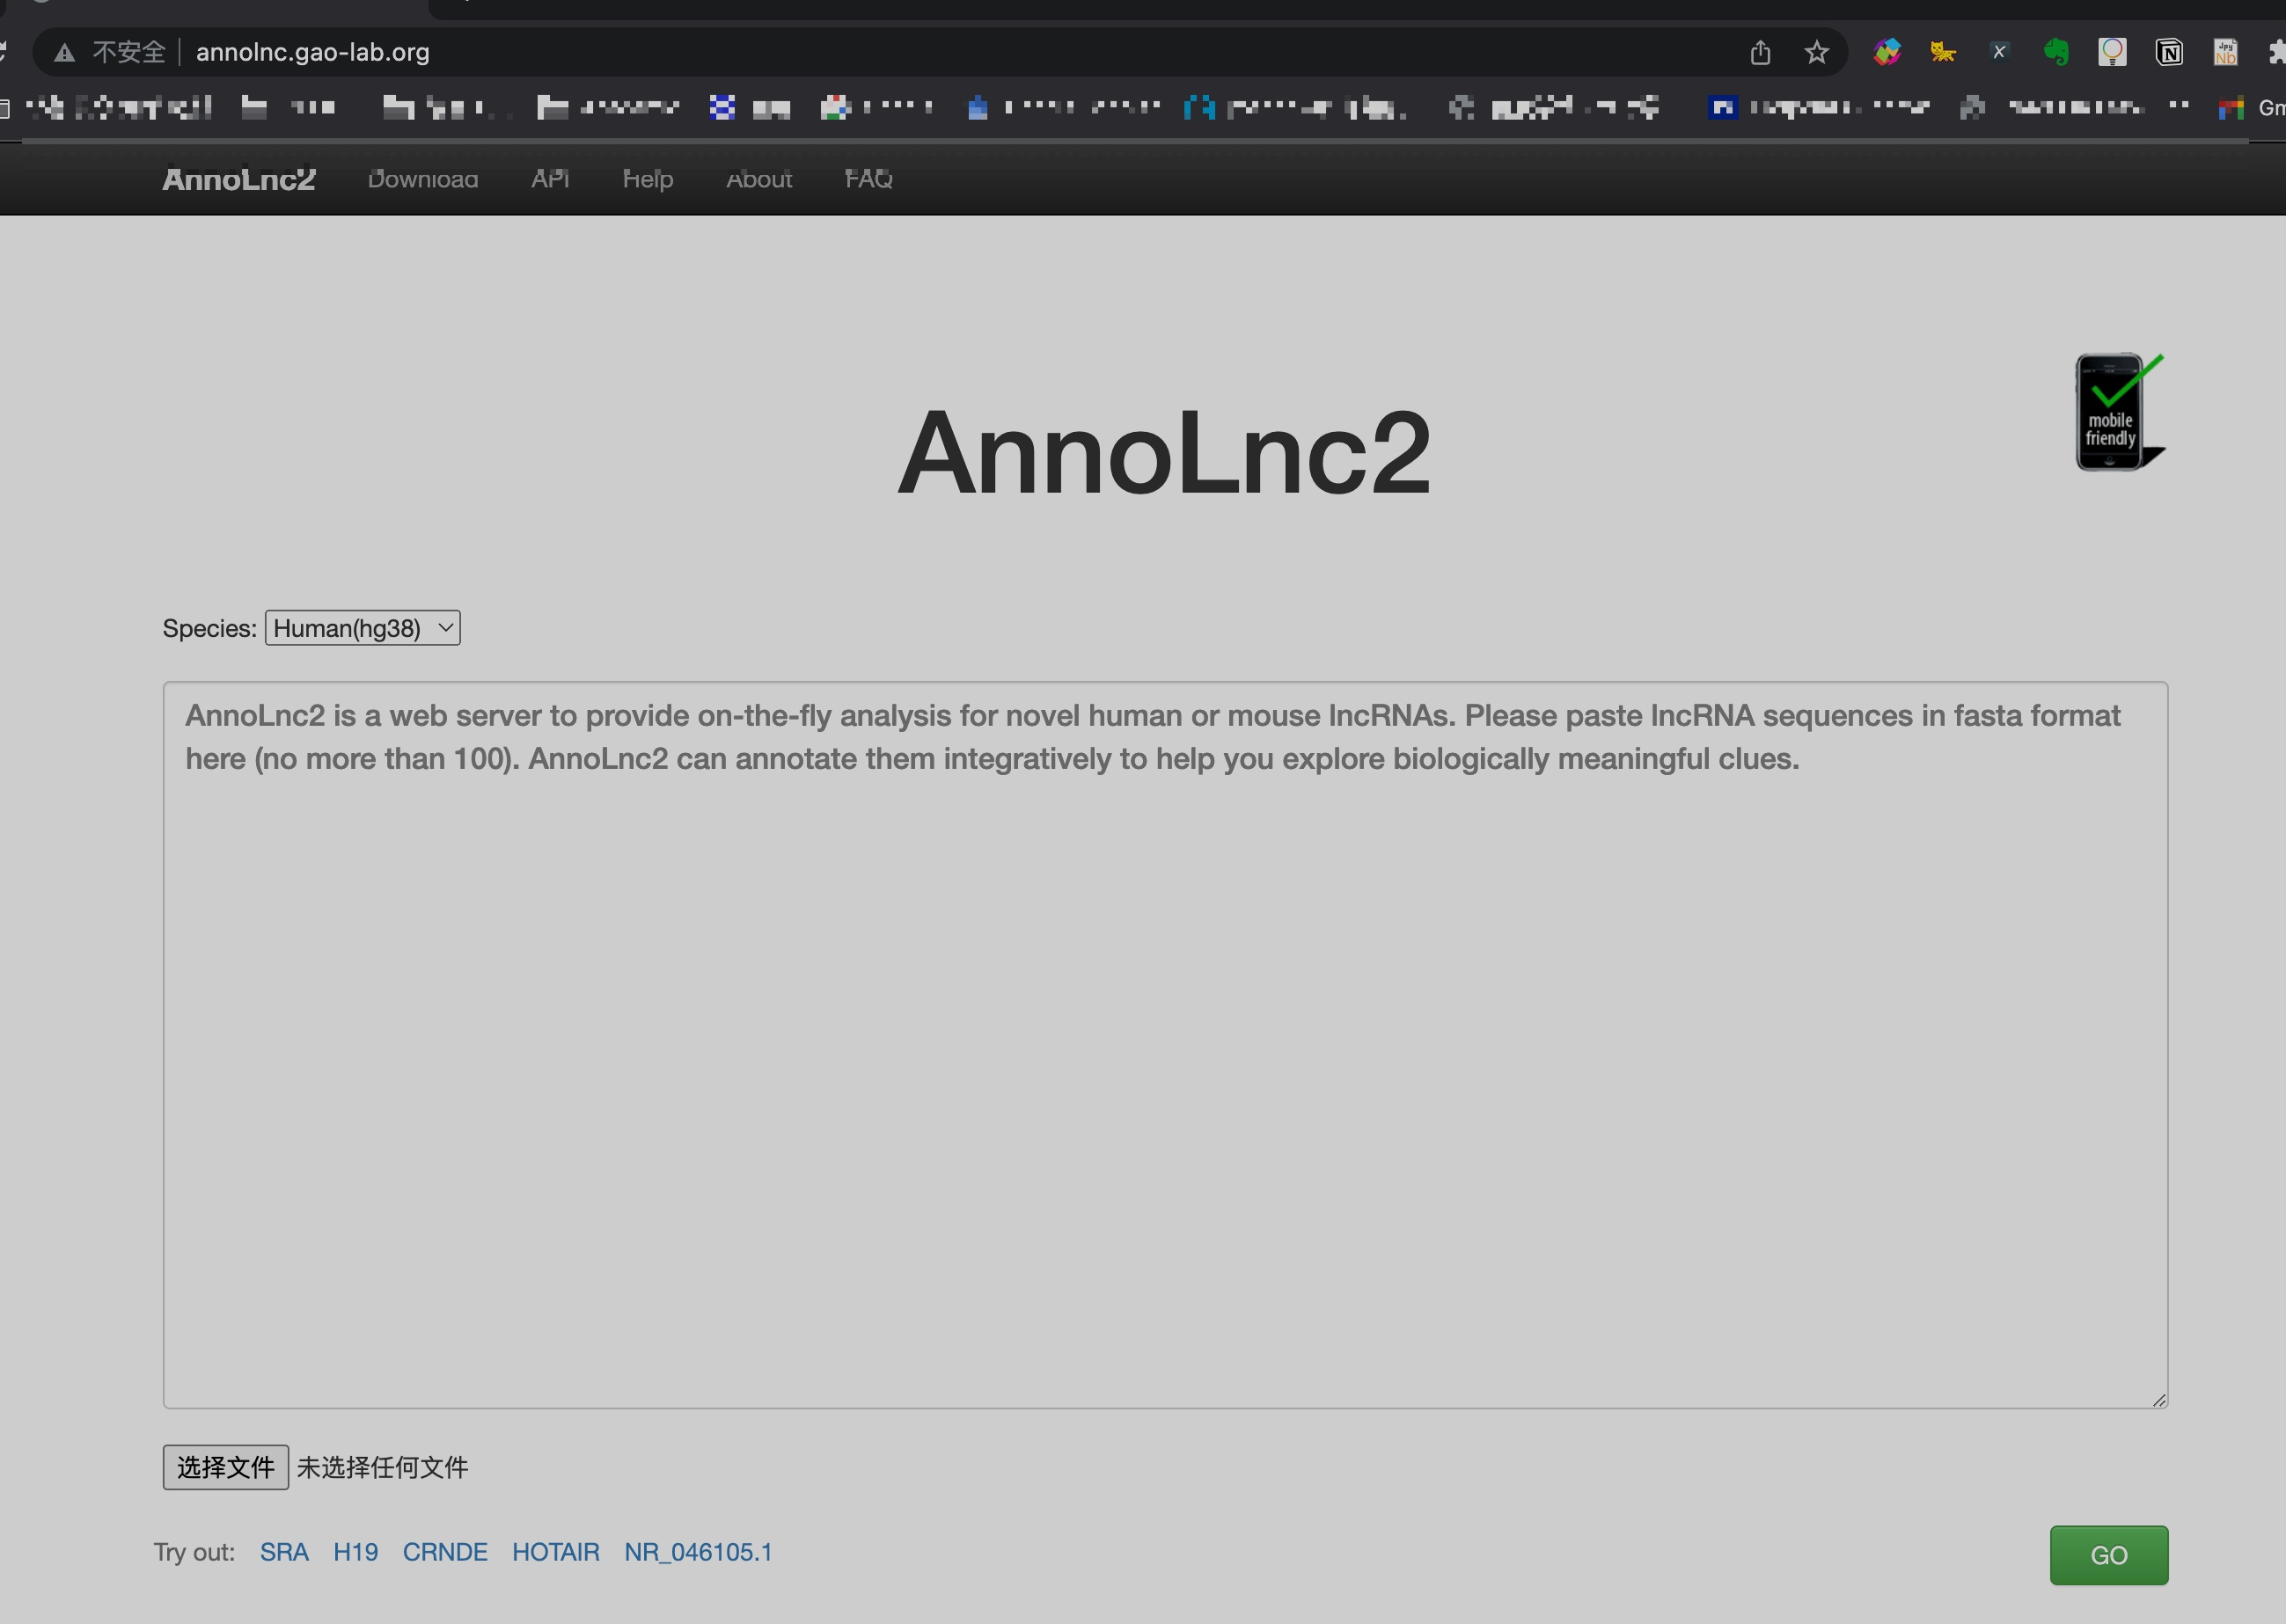
\includegraphics[width=8cm]{Images/annolnc2.jpg}
            \caption{AnnoLnc2 lncRNA 网页端分析工具}
        \end{figure}
    \end{columns}

\end{frame}

% 再比如, 北京大学的高歌老师课题组使用 Python 开发了一个网页端的生物信息学分析工具
% 叫做 AnnoLnc2, 你看名字就知道这个工具可以用来进行 LncRNA 相关的分析

\begin{frame}{Python在生物信息学中的应用}
    \begin{myoutline}[itemize]
        \1 数据获取
            \2 \textcolor{lightgray}{爬虫}
        \1 \textcolor{lightgray}{Web前后端开发}
            \2 \textcolor{lightgray}{Django, Flask, 数据库\dots}
        \1 工作流程
            \2 Jupyterlab
            \2 \textcolor{lightgray}{Snakemake}
        \1 字符串处理 \textcolor{red}{(强项)}
            \2 FASTA, FASTQ, BED-like, BAM/SAM
            \2 \underline{Biopython, Pysam}
        \1 数据分析机器学习
            \2 数据清洗, 数据分析, 可视化
            \2 \textcolor{lightgray}{特征工程, 机器学习}
    \end{myoutline}
\end{frame}

% 其实 Python 一个特性就是它是对字符串进行处理的能力非常强大
% 而很多生物信息学文件格式都是以文本为基础的格式
% 而使用 Python,就能比较容易的对这些文本文件进行处理
% 字符串处理也是我们这门课程的核心内容
% 而同时 Python 中也有比如 Biopython 和 Pysam 的第三方包
% 也可以使用这些包来对序列文件和 BAM 文件进行比较好的处理
% 最后就是, Python 中的 Jupyterlab 这个 IDE 工具,以后我会详细讲, 
% 它可以帮助我们进行数据分析和项目管理
% 而 Snakemake 就是基于 Python 编写的一个命令行的流程控制工具,
% 在生物信息学分析流程的标准化中有非常广泛的应用

% 这里标灰色的部分我们这门课暂时不涉及,而黑色字体所述的内容,在后面的课程内容中都会涉及

% 好,我们简单介绍完了 Python 的发展历程和Python 能够做的事情
